\documentclass[a4paper,14pt]{extarticle} 
\usepackage[a4paper,top=1.5cm, bottom=1.5cm, left=2cm, right=1cm]{geometry}
%\usepackage[T2A]{fontenc}
%\usepackage[english, russian]{babel}
\usepackage{graphicx}
\graphicspath{{./pics/}}
\DeclareGraphicsExtensions{.pdf,.png,.jpg}

\usepackage{fontspec}
\setmainfont{Times New Roman}
\setsansfont{FreeSans}
\setmonofont{FreeMono}
\renewcommand{\baselinestretch}{1.5}
\usepackage{polyglossia}
\setdefaultlanguage{russian}
\setotherlanguages{english,russian}
\usepackage{setspace}
\usepackage[many]{tcolorbox}

\begin{document}

    \begin{center}
        \thispagestyle{empty}
        \begin{singlespace}
        ФЕДЕРАЛЬНОЕ АГЕНТСТВО СВЯЗИ

        ФЕДЕРАЛЬНОЕ ГОСУДАРСТВЕННОЕ БЮДЖЕТНОЕ ОБРАЗОВАТЕЛЬНОЕ

        УЧРЕЖДЕНИЕ ВЫСШЕГО ОБРАЗОВАНИЯ

        «САНКТ-ПЕТЕРБУРГСКИЙ ГОСУДАРСТВЕННЫЙ УНИВЕРСИТЕТ ТЕЛЕКОММУНИКАЦИЙ ИМ. ПРОФ. М.А. БОНЧ-БРУЕВИЧА»

        (СПбГУТ)
        \end{singlespace}
        \vspace{-1ex}
        \rule{\textwidth}{0.4pt}
        \vspace{-5ex}

        Факультет \underline{Инфокоммуникационных сетей и систем}

        Кафедра \underline{Защищенных систем связи}
        \vspace{10ex}

        \textbf{Лабораторная работа №4}

    \end{center}
    \vspace{4ex}
    \begin{flushright}
    \parbox{8cm}{
    \begin{flushleft}
        Выполнил:

        \underline{Громов А.А., ИКТЗ-83} \hfill \rule[-0.85ex]{0.1\textwidth}{0.6pt}\\
        \vspace{-1ex}
        \footnotesize \textit{ (Ф.И.О., № группы) \hfill (подпись)} \normalsize

        Проверил:

        \underline{Гельфанд А.М.} \hfill \rule[-0.85ex]{0.1\textwidth}{0.6pt}\\
        \vspace{-1ex}
        (\footnotesize \textit{уч. степень, уч. звание, Ф.И.О.) \hfill (подпись)} \normalsize

    \end{flushleft}
    }
    \end{flushright}
    \begin{center}
        \vfill
        Санкт-Петербург

        2020

        \end{center}

    \newpage
    \begin{center}
        \textbf{\large{ Введение}}
    \end{center}
    Цель работы:\par 
    Целью данной лабораторной работы является получение базовых навыков по 
    работе с командным интерфейсом коммутаторов Cisco. 
    Рассматриваютсяприемы первичной настройки коммутаторов, обеспечения их 
    защищенностии доступности для управления.\\

    Схема сети:\\
    \begin{center}
        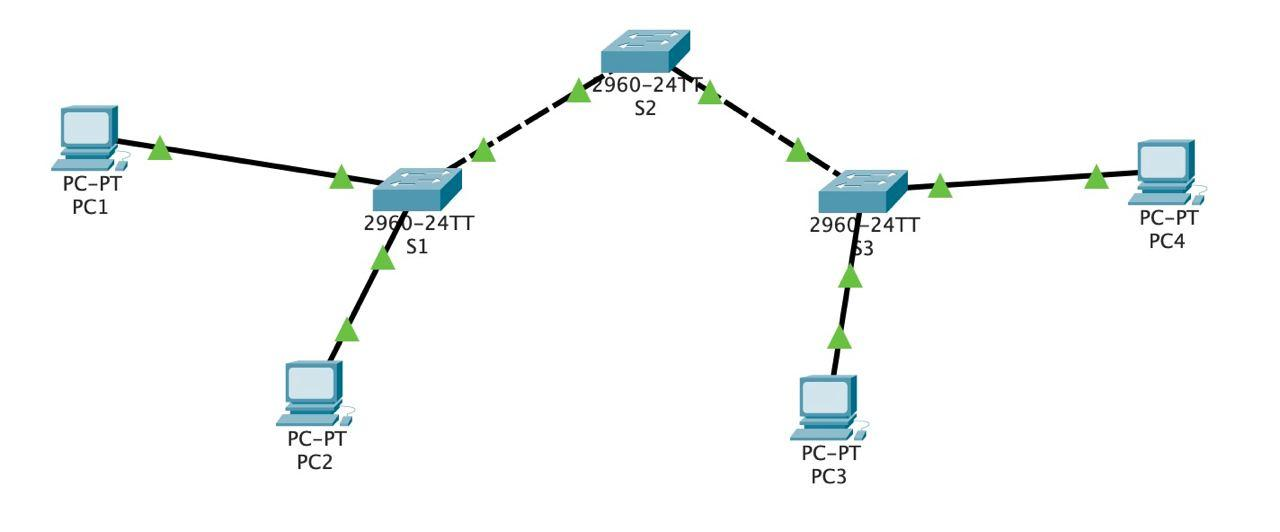
\includegraphics[scale=0.5]{1.jpg}
    \end{center}
    
    Смена имени коммутатора, а так же установка пароля к привилегированному
    режиму на коммутаторе. 
    \begin{center}
        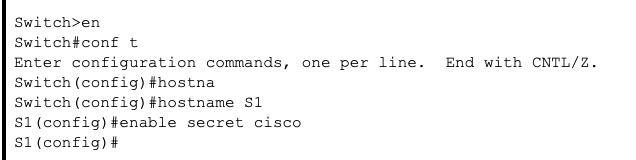
\includegraphics{5}
    \end{center}
    \newpage
    \par Настройка ip-адреса и маски на коммутаторе.
    \begin{center}
        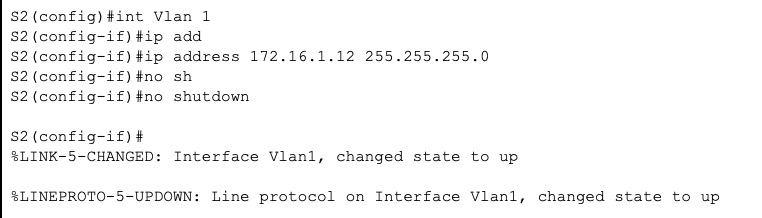
\includegraphics[scale=0.8]{4.jpg}
    \end{center}
    \par Установка ip-адреса и маски на персональном компьютере.
    \begin{center}
        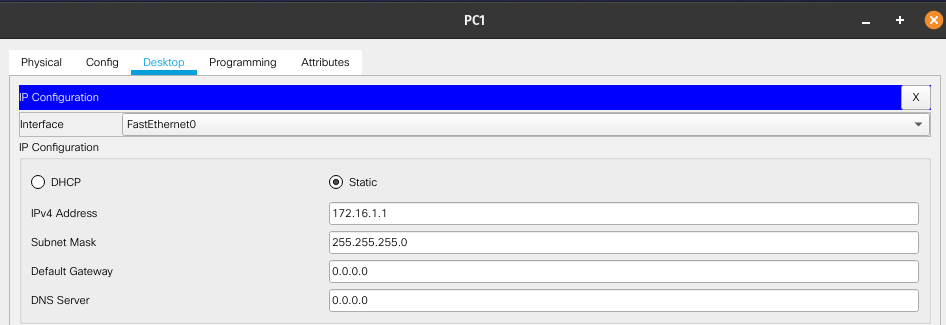
\includegraphics[scale=0.5]{6.png}
    \end{center}
    \par Проверка соединения:
    \begin{center}
        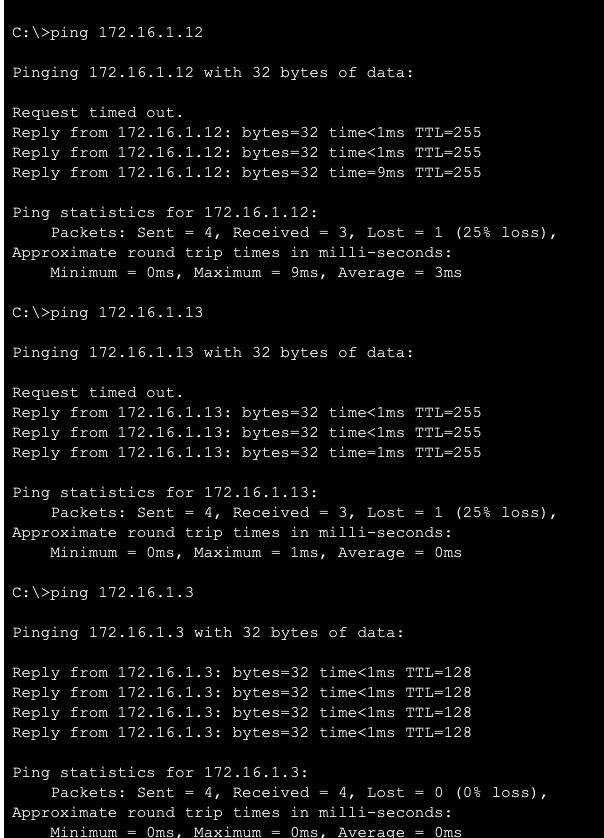
\includegraphics[scale=0.5]{3}
    \end{center}
    \par Режим симуляции:
    \begin{center}
        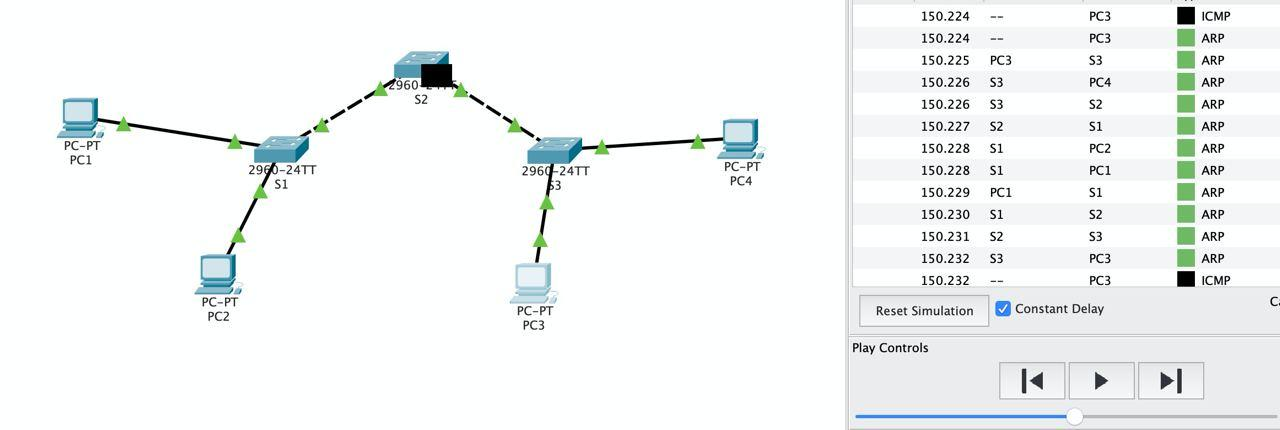
\includegraphics[scale=0.5]{2.jpg}
    \end{center}
    \par В данном случае команда ping запускалась впервые. Так как у нас локальная 
    сеть, данные передаются на 2 уровне(кадры). Для передачи информации на 2ом
    уровне требуется знать mac-адрес устройства получателя. Для это производится
    широковещателный запрос в сети. Как только мы узнали mac-адрес устройства
    получателя, мы сопоставляем его с ip-адрсом и отсылаем уже icmp запросы.
    ICMP-протокол является служебным протоколом, и в основном используется для
    выявления ошибок в сети.\\\par
    \textbf{Вывод:}\par 
    В ходе данной лабораторной работы я научился настраивать небольшую 
    локальную сеть и выполнять базовую настройку коммутаторов и компьютеров.
    Также я ознакомился с работой ICMP, ARP протоколов и тем, какой трафик
    передается по сети в ходе их работы.
\end{document}